%!TEX TS-program = xelatex
%!TEX encoding = UTF-8 Unicode
% !TEX root = ../../metm.tex

\chapter{STEREOFONIA}
\startcontents[chapters]
\printcontents[chapters]{}{1}{}

\vfill\null

Il primo passo necessario nella comprensione del concetto di \emph{Stereofonia},
prima di arrivare alle tecniche ed alle tecnologie elettroacustiche che la
rendono possibile, è stabilire attraverso l'etimologia del termine e dei
termini ad esso collegati una base concettuale solida. \emph{Stereo}, dal greco
\emph{Stereos}, significa \emph{solido}. Non un numero, non una configurazione
ma un aggettivo qualitativo. Nel dizionario inglese Oxford: \emph{Solid, firm
and stable in shape. Having Three dimension}. Solido, \emph{solid}, dalla radice
latina di \emph{Solidus, Sollus}, intero.

Con la parola \emph{Stereofonia} dovremmo quindi descrivere una condizione
nella quale \emph{phon\={e}}, sempre dal greco, \emph{suono}, la \emph{voce},
arrivi all'ascoltatore solida, integra, ferma e stabile nella sua forma (sonora)
multi dimensionale, intera.

\clearpage

%%%%%%%%%%%%%%%%%%%%%%%%%%%%%%%%%%%%%%%%%%%%%%%%%%%%%%%%%%%%%%%%%%%%%% LE RADICI
%%%%%%%%%%%%%%%%%%%%%%%%%%%%%%%%%%%%%%%%%%%%%%%%%%%%%%%%%%%%%%%%%%%%%%%%%%%%%%%%
\section{LE RADICI}

Indispensabile alla comprensione del mondo sonoro elettracustico, nelle sue
radici, è anche la descrizione di \emph{mono}, nomignolo di \emph{monofonico},
espresso nel legame tra \emph{monos} e \emph{phon\={e}}: una voce,
\emph{one voice}, \emph{alone}, sola. La stessa parola usata nella descrizione
del canto gregoriano, successivamente evolutasi in \emph{polifonia} (dal greco
\emph{poluph\={o}nia}, da \emph{polu}, molte, \emph{many} e \emph{phon\={e}},
voci). Quindi la dicotomia, se proprio deve essercene una, tra monofonia e
stereofonia semplicemente non esiste. L'estensione del concetto di monofonia,
nel suo eventuale opposto, è polifonia. La stereofonia è semplicemente un
concetto altro.

Con la parola stereofonia dovremmo descrivere anche la condizione in base alla
quale il suono arrivi \emph{solido} all'ascoltatore, \emph{intero, fermo e
stabile} nella sua forma sonora multidimensionale originaria, attraverso
la riproduzione elettroacustica, attraverso la trasmissione e la diffusione con
gli altoparlanti, con un numero qualsiasi, o necessario, di canali.

\vfill\null

%------------------------- APPROFONDIMENTO
\begin{tabular}{L{.969\textwidth}}%
\toprule
	\textbf{Alan Dower Blumlein}\\
\midrule
Nato il 29 giugno 1903 a Londra, Deceduto il 7 giugno 1942 a Herefordshire,
Inghilterra, fu ingegnere elettronico presso EMI, per la quale pubblicò brevetti
per le sue numerose invenzioni nel campo delle telecomunicazioni soprattutto in
relaizone alle tecnologie di registrazione, trasmissione e diffusione del suono.
Ottiene, nella sua breve carriera, 128 brevetti, motivo per cui è considerato
uno dei più importanti ingegneri e inventori del suo tempo. Morì durante la
seconda guerra mondiale all'età di 38 anni, durante un test militare segreto del
sistema radar H2S allora in fase di sviluppo, a bordo del bombardiere Halifax
su cui stava volando. Tra le numerose invenzioni legate al nome di Blumlein
quelle legate alla Stereofonia stravolsero completamente il mondo della
fruizione pubblica del suono. Le sue prime note sull'argomento risalgono al 25
settembre 1931 e il suo brevetto aveva il titolo “Miglioramenti ai, ed in
relazione ai, sistemi di trasmissione, registrazione e riproduzione del suono”.
La domanda di brevetto fu del 14 dicembre 1931 ed la concessione fu dell
14 giugno 1933, brevetto britannico numero 394.325.\\
\bottomrule
\end{tabular}
%------------------------- APPROFONDIMENTO

\clearpage

La percezione dei caratteri spazio-temporali dei suoni, in particolare della
loro direzione di provenienza e della loro relazione con lo spazio che
attraversano, definiscono i tratti essenziali della stereofonia, in relazione
all'udito, in virtù dell’audizione biauricolare (o binaurale). Come sottolineato
nell'enciclopedia Treccani, tra le varie definizioni di stereofonia \emph{il
termine è inoltre usato per indicare la parte dell’acustica fisiologica
che si occupa di tale fenomeno}. L'ascolto biauricolare del sistema uditivo
conferisce alla percezione umana il potere localizzatore, cioè la capacità,
dovuta al lavoro congiunto dei due sistemi auricolari separati ed al sistema
nervoso centrale, di determinare la direzione di provenienza di un suono. In tal
senso, esiste in acustica fisiologica la definizione di monofonia in qualità di
condizione anomala del sistema percettivo, caratterizzata dalla mancanza degli
elementi necessari a individuare i caratteri spaziali dei suoni stessi, come per
esempio quella ottenuta con un solo orecchio.

L'ultimo esercizio linguistico è legato alla definizione dell'aggettivo
\emph{stereofònico} e ci permette di aprire il termine alle tecniche ed alle
tecnologie che hanno reso possibile la trasmissione, la riproduzione,
e la diffusione della stereofonia. \emph{Stereofònico}, quindi, che si riferisce
alla stereofonia, alla percezione della stereofonia, alla descrizione delle
tecniche di registrazione e riproduzione in grado di operare stereofonia. Un
aggettivo che dovrebbe essere usato solo nella
descrizione di tecniche di registrazione e di diffusione sonora atte alla
riproduzione dei suoni in modo che l’ascoltatore abbia l’impressione di trovarsi
nello spazio sonoro originale, dai quali ne deriva una musica stereofonica ed
una discografia stereofonica in grado di grarantire l’ambiente sonoro originale,
solido e tridimensionale attraverso l’effetto stereofonico.

\begin{quotation}
An observer in the room is listening with two ears, so that echoes reach him
with the directional significance which he associates with the music performed
in such room. He therefore discount these echoes and psychologically focuses
his attention on the source of the sound. When the music is reproduced through
a single channel the echoes arrive from the same direction as the direct sound
so that confusion results. [\ldots] Human ability to determine the direction
from which sound arrives is due to binaural hearing, the brain being able to
detect differences between sound received by the two ears from the same source
and thus to determine angular directions from which various sounds
arrive\footnote{Un osservatore nella stanza sta ascoltando con due orecchie, in
modo che gli echi lo raggiungano con il significato direzionale che associa alla
musica eseguita in quella stanza. Pertanto, non tiene conto di questi echi e
focalizza psicologicamente la sua attenzione sulla fonte del suono. Quando la
musica viene riprodotta attraverso un singolo canale, gli echi arrivano dalla
stessa direzione del suono diretto, in modo da creare confusione. [...] La
capacità umana di determinare la direzione da cui proviene il suono è dovuta
all'udito binaurale, il cervello è in grado di rilevare le differenze tra il
suono ricevuto dalle due orecchie dalla stessa fonte e quindi di determinare le
direzioni angolari da cui provengono i vari suoni.}. [\cite{ab58}]
\end{quotation}

Con queste parole Blumlein nel 1931 descrive i fondamenti di almeno due grandi
argomenti: quali erano le conoscenze  dell'epoca su come percepiamo i suoni
acustici e come abbiamo riprodotto i suoni fino a quel momento.

La binauralità dell'ascolto umano è la prima affermazione di Blumlein:
“\emph{un osservatore nella stanza sta ascoltando con due orecchie}”. Come
questa condizione di ascolto si evolva nel tempo è la peculiarità della
stereofonia.

% Non è correlato al numero di fonti, nemmeno al numero di microfoni
% e altoparlanti necessari per riprodurre tale condizione. La tecnica e lo scopo
% della tecnica prescelta si concentreranno per risolvere più argomenti possibili
% per soddisfare tale condizione.

%%%%%%%%%%%%%%%%%%%%%%%%%%%%%%%%%%%%%%%%%%%%%%%%%%%%%%%%%%%%%%%%%%%%%%%%%%%%%%%%%%%%%%%%%%%%%%%%%% dalle esposizioni
Dovremmo indicare quindi qualitativamente una condizione di ascolto, dal latino
\emph{auscultare}, prestare attenzione a qualcosa in quanto oggetto o motivo di informazione, con specifiche caratteristiche di solidità spaziale, dimensionalità osservabili nella forma sonora riconoscibile, informativa.

\emph{Una voce in una piccola stanza riverberante è una condizione d'ascolto che
rispetti queste qualità?}

Prima di approfondire questioni di propagazione e percezione del suono, val la pena
dedicare un tempo alla letteratura specializzata.

\begin{quote}
When recording music considerable trouble is experienced with the unpleasant
effects produced by echoes wich in the normal way would not be noticed by anyone
listening in the room in which the performance is taking place. An observer in
the room is listening with two ears, so that echoes reach him with the directional
significance which he associates with the music performed in such room. He,
therefore, discounts these echoes and psychologically focuses his attention on
the source of the sound\footnote{Quando si registra musica acustica, si riscontrano
notevoli problemi a causa degli effetti indesiderati prodotti dalle riflessioni
acustiche dell'ambiente, che nell'ascolto normale non vengono notati dagli
ascoltatori nella stanza in cui si svolge l'esibizione. L'ascoltatore, nella stanza,
ascolta attraverso le due orecchie, le riflessioni lo raggiungano con il significato direzionale che associa alla musica eseguita in quella stanza.
Pertanto, elimina dal messaggio le informazioni delle riflessioni e focalizza
psicologicamente la sua attenzione sulla sorgente sonora.}.
\end{quote}

Richiesta di brevetto numero 394325 del 14 dicembre 1931, accettazione del 14
giugno 1933. Alan Dower Blumlein.

La risposta alla domanda \emph{Una voce in una piccola stanza riverberante è una
condizione d'ascolto che rispetti queste qualità?} è, in funzione di quanto
appena letto, chiaramente affermativa.

Anche con un solo oggetto sonoro, una sola voce, in una piccola stanza, siamo in
presenza di un fenomeno acustico stereofonico. Almeno così dice Blumlein, papà
della stereofonia, nel brevetto in cui ne rende i concetti fondamentali, solidi,
stabili nel tempo e nello spazio delle parole, nel brevetto tecnologico che stabilisce
il \emph{point break} dell'elettroacustica, per il resto dell'umanità.

\begin{figure}[h]
\begin{center}
  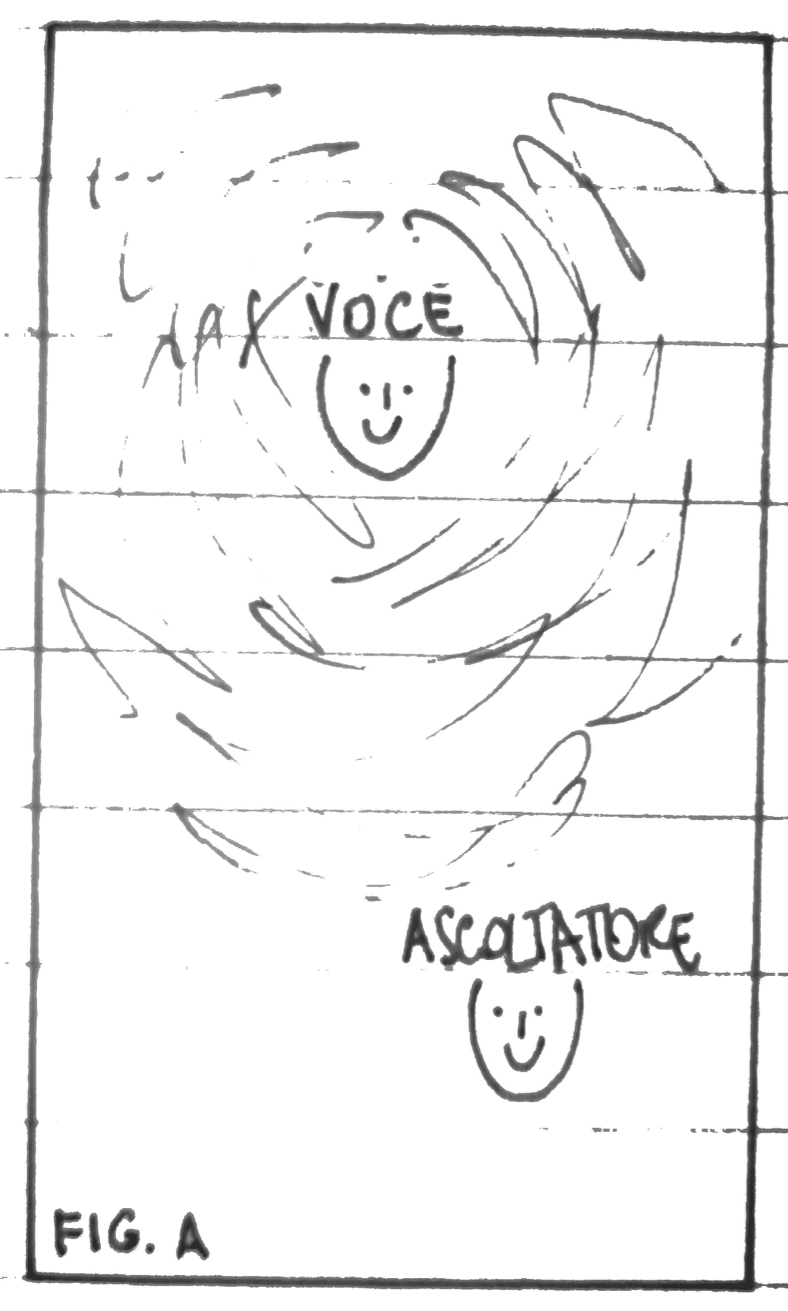
\includegraphics[width=.48\linewidth]{CAPITOLI/1000/IMG/figa.png}
%\caption{}
\label{ee:figa}
\end{center}
\end{figure}

Una voce nello spazio di una stanzetta si dirige, con una sua direzione, verso
un punto e contemporaneamente, con meno direzionalità, lateralemente, raggiunge
il resto della stanza. Questo meccanismo ha a che fare con la forma sonora di una
voce, prima ancora che con la forma architettonica della piccola stanza.

Dobbiamo immaginare la forma sonora come un'armatura attorno al nostro oggetto
sonoro, un'armatura fatta di fittissime molecole in vibrazione. Ogni suono ha una
sua veste plastica. Se vi dicessi ottavino e poi contrabbasso voi avreste già
collegato tutto ciò che vi serve per vederli, sentirli, ed ora, volendo, vestirli
della loro forma sonora. Ma cosa accade alla forma sonora di uno strumento in
presenza di tecninche estese applicate allo strumento? Una mano che inizia a produrre
suono li, nello stesso luogo dello strumento, a dove pochi minuti prima premeva
solo tasti (la mano  sinistra di UR) diventa esplosione di forma acustica e musicale.

Ecco questo è un po' il cuore di quello che vorrei fosse il mio dottorato di
ricerca che non avrò mai e un po' anche la manifestazionne di una piuttosto
triste verità: esclusi i percorsi individuali e rari percorsi di ricerca
non istituzionalizzata, la musica contemporanea ha esaurito la sua carica
contributiva al conoscimento, alla comprensione generalizzata.

Tornando alla forma, Questa si staglia nello spazio circostante e si espande e si muove
all'interno di questo spazio e ne viene modellata come una massa morbida all'interno
di un contenitore. Qui iniziano i fenomeni di riflessione e la forma si
cristallizza assumendo caratteristiche in funzione dello spazio e, quindi, del tempo.
L'ascoltatore che partecipa a questo evento vede una persona solida parlare nello
spazio di una stanza e sente la forma solida della voce provenire dalla sua bocca
e contemporaneamente, quindi subito dopo, dalla stanza sotto forma di riflessioni.
Sì! converremo infine, questa esperienza di ascolto rispetta queste qualità.

\begin{figure}[h]
\begin{center}
  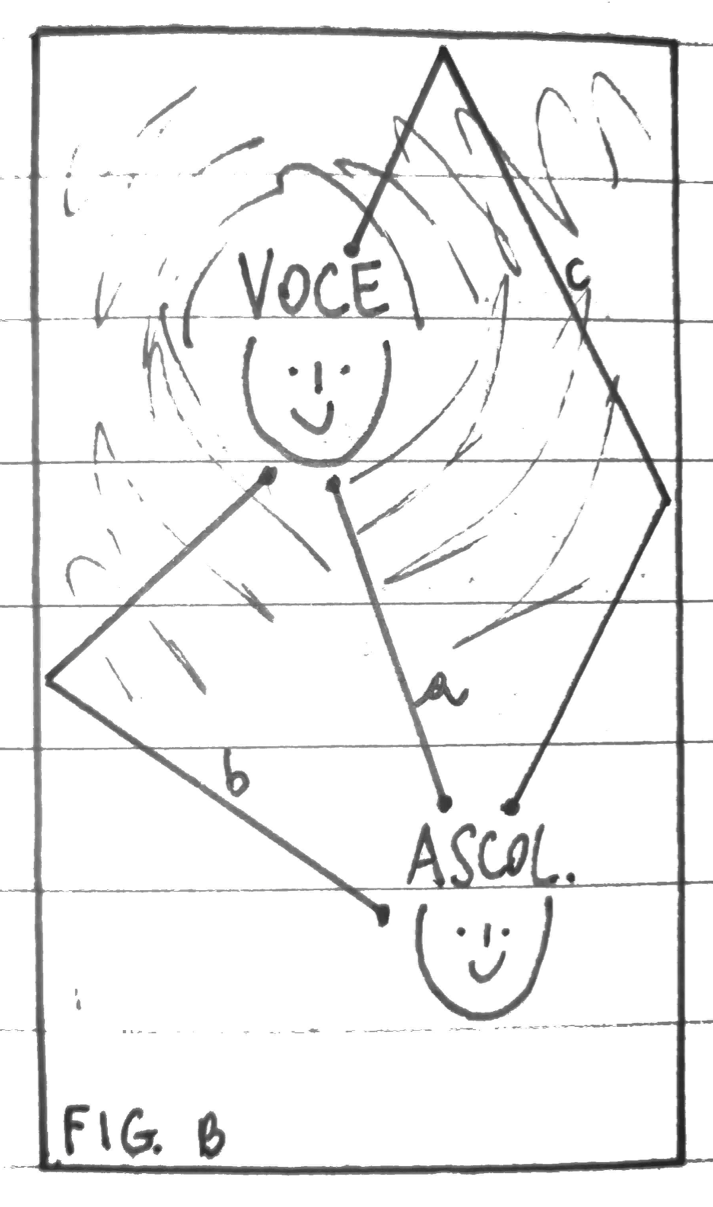
\includegraphics[width=.48\linewidth]{CAPITOLI/1000/IMG/figb.png}
%\caption{}
\label{ee:figa}
\end{center}
\end{figure}

Una voce che attraverso la sua forma acustica riempia uno spazio acustico è
un'esperienza d'ascolto stereofonica. Non è ancora giunto il momento di
interrompere la discussione dicendo: “ma come, non servono due diffusori?” Non
ancora, il problema è più complesso. È importante sottolineare che la stereofonia,
l'ascolto stereofonico, è una qualità dell'ascolto che si può osservare in
determinate circostanze e che richiede necessariamente il lavoro concertato delle
due orecchie. Un ascolto stereofonico è quindi possibile solo in coincidenza
con un ascolto \emph{binaurale}, ovvero effettuato con entrambe le orecchie.

Di nuovo una qualità che presuppone dei contenuti coerenti con delle
caratteristiche specifiche. Ora, nel mondo elettroacustico, del suono prodotto
o riprodotto elettricamente, dovremmo essere in grado di effettuare lo stesso
ragionamento sostituendo alla persona che parla un diffusore generico. Come per
l'essere umano, la voce è esempio di suono proprietario anche per il diffusore
si può scegliere un suono che lo caratterizzi elettroacusticamente, un suono
che lo rende particolare: il suono definito rumore rosa. Posizionato il diffusore
nella stessa stanza e con le stesse circostanze di ascolto precedenti, avremmo
una condizione di ascolto stereofonico? Ovviamente si. Un solo diffusore può
costituire una condizione d'ascolto stereofonica. In questo caso l'oggetto
acustico è un diffusore che esprime se stesso attraverso un suono non informativo.
Un rumore è caratterizzato da un'assenza di informazione, fatta esclusione del
fatto stesso che è rumore.

\begin{figure}[h]
\begin{center}
  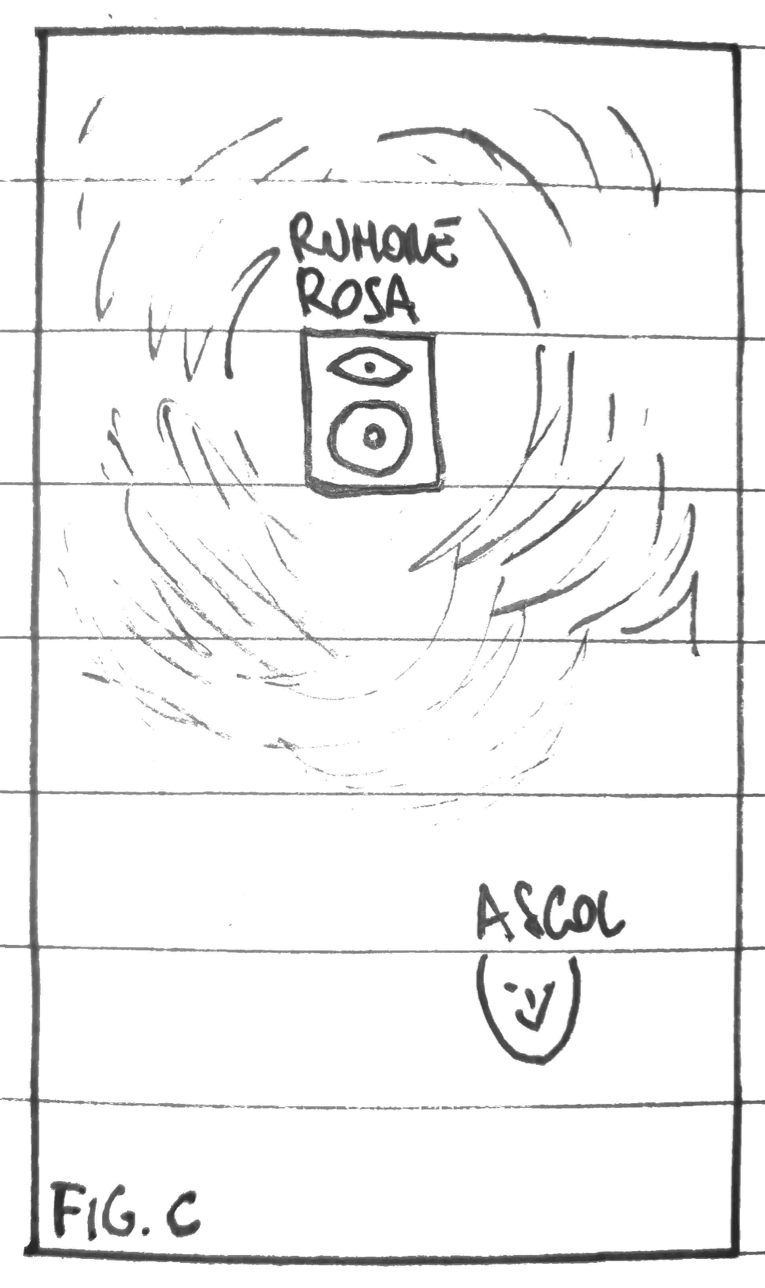
\includegraphics[width=.48\linewidth]{CAPITOLI/1000/IMG/figc.png}
%\caption{}
\label{ee:figa}
\end{center}
\end{figure}

che informazioni? be quelle che descrivono un suono come la percezione di altezza,
durata, intensità e timbro. Questa descirizione di stereofonia possibile anche
con un solo soggetto sonoro, voce o diffusore che sia, non è così comune e
condivisa. Ciò accade a causa del fatto che spesso si fa confusione tra stereofonia,
o stereofonica, come aggettivo applicato alla tecnica di diffusione e registrazione
piuttosto che alla qualità percettiva che queste tecniche dovrebbero suggerire.

Per arrivare a descrivere la tecnica dobbiamo percorrere ancora alcuni passi.

Nel momento in cui si passa da un dominio puramente acustico sia esso derivante
da una voce umana quanto un rumore diffuso attraverso un altoparlante, ad un
dominio di riproduzione acustica, ovvero di rappresentazione attraverso meccanismi
e tecniche allora cambia completamente lo scenario acustico e le circostanze di
ascolto. Un diffusore tradizionale può riprodurre una voce umana o un diffusore
che suona rumore rosa? Si certo che può riprodurli. Questa riproduzione
costituirebbe un ascolto stereofonico della sorgente originale? No, non lo sarebbe.

\begin{figure}[h]
\begin{center}
  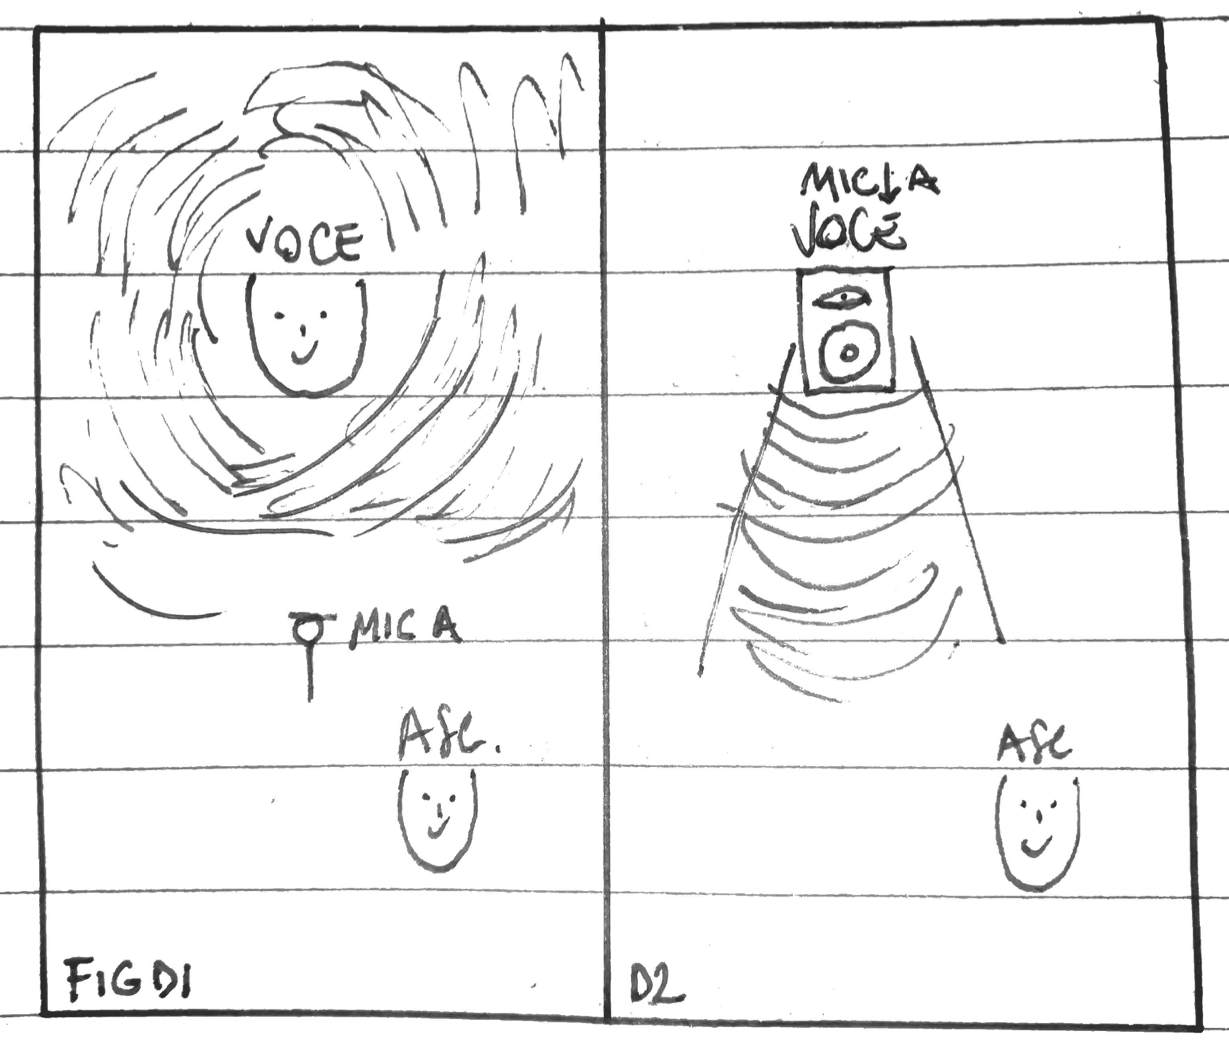
\includegraphics[width=.98\linewidth]{CAPITOLI/1000/IMG/figd1d2.png}
%\caption{}
\label{ee:figa}
\end{center}
\end{figure}


\begin{quote}
When the music is reproduced through a single channel the echoes arrive from the same direction as the direct sound so that confusion result\footnote{Quando la musica viene riprodotta attraverso un singolo canale, gli echi arrivano dalla stessa direzione del suono diretto in modo tale da creare confusione.}.
\end{quote}

Qui si sviluppa tutta la questione, un solo diffusore non è in grado di rappresentare
la solidità originaria, la forma sonora dell'oggetto acustico originario, il suo
rapporto con lo spazio che lo ha modellato. Per comprendere meglio ogni possibile
questione legata alla diffusione sonora, mediante dispositivi elettroacustici ci
vorrebbe un minimo di tempo speso nella sperimentazione con lo strumento altoparlante.
Perché di questo si parla, di uno strumento tecnico, tecnologico, musicale e
profesisonale.

\begin{quote}
Ci sono problemi che alle volte anch'io non capisco, nel senso che se ne porgono
continuamnte di nuovi. È da anni che lavoro e sperimento negli studi di live electronics di
Friburgo, della Sudwestfunk. Si tratta delle trasformazioni in tempo reale del
suono e della voce, e del comporla con lo spazio, usando le tecnologie di oggi,
con i vari altoparlanti disposti nella sala. C'è qualcosa di nuovo solo sul piano
tecnico, perché  se prendiamo la Scuola di S. Marco veneziana di Andrea e Giovanni
Gabrieli, Monteverdi, di Willaert, con le composizioni a più cori, la grande
scuola spagnola all'epoca di Filippo II [\ldots] si faceva musica per otto organi
e quattro cori, cioè si suonava lo spazio come componente musicale, non come poi
la prassi dell'ottocento usa lo spazio, mettendo dentro l'orchestra e quel che
succede succede. Quindi altri studi, anche studi di fisica architettonica, studi
di processi di eco, di riverberazione, di materiali acustici. [\ldots] Qui una
composizione non è  data una volta per sempre, perché per ogni spazio noi dobbiamo
cambiare i programmi dei computer e modificando i rapporti della trasformazione si modifica anche il rapporto acustico; [\ldots] il grande fascino di questo per me
è veramente la non ripetitività. [\ldots] Un interprete non deve studiarsi la
parte ma veramente partecipare. [\ldots] Cioè vedi come noi possiamo con la
tecnologia di oggi studiare molto meglio, cioè studiare in un altro modo. \\
Luigi Nono 1986
\end{quote}

La parabola bacchiana si conclude con una nota autobiografica. Noi, che abbiamo
osservato da vicino la maledizione di Bacco, non possiamo più tacere e seminiamo,
il vento muoverà le orecchie penzolanti e porterà le nostre confessioni altrove.
%%%%%%%%%%%%%%%%%%%%%%%%%%%%%%%%%%%%%%%%%%%%%%%%%%%%%%%%%%%%%%%%%%%%%%%%%%%%%%%%%%%%%%%%%%%%%%%%%% fiune dalle esposizioni

Una singola voce umana, monofonica, sta parlando all'interno di una piccola
stanza, una condizione stereofonica accettabile? In accordo con Blumlein,
Sì! Questo è il primo punto fermo.

Michael Gerzon, dagli anni settanta agli anni novanta, dalle radici dell'era di
Blumlein ha saltato la linea con una dozzina di descrizioni chiare sulla
percezione e tentativi di progettare tecnologie di riproduzione per colmare il
divario rispetto al regno acustico.

\begin{quotation}
The ears and brain localize sounds according to many different mechanism. Among
the most important cues used are low frequency interaural phase (applicable up
to around 2\emph{KHz}, but dominant below 700\emph{Hz}) and localization by
amplitude differences between the two ears, predominantly above about
1\emph{KHz}. While other cues are also important, we have found that satisfying
both these cues, and making them mutually consistent for central listener facing
in any direction, leads to particularly robust and reliable localization
quality.\cite{mg92pdmsss}
\end{quotation}

%%%%%%%%%%%%%%%%%%%%%%%%%%%%%%%%%%%%%%%%%%%%%%%%%%%%%%%%%%%%%%%%%%% SECTION FOUR
%%%%%%%%%%%%%%%%%%%%%%%%%%%%%%%%%%%%%%%%%%%%%%%%%%%%%%%%%%%%%%%%%%%%%%%%%%%%%%%%
\section{RAMIFICAZIONI}

Con la profonda conoscenza del significato del tempo tra noi e Blumlein,
possiamo esporre il significato degli altoparlanti meglio di lui. Per l'era
Blumlein, l'altoparlante era lo strumento futuro per un tempo presente migliore.
Il suono riprodotto, alla sua giovane età, era pura magia. Oggi sappiamo bene
quanto siamo insoddisfatti della riproduzione degli altoparlanti. Quando il
primo iPhone è stata l'unica cosa intelligente sul pianeta, è stato fantastico,
un fantastico oggetto di creazione. Oggi con lo stesso oggetto non faremmo
nemmeno una foto. Ascoltare un assolo di violino riprodotto dal miglior
altoparlante sul mercato non è la stessa esperienza della performance reale.
Non è legato alla stereofonia e all'abilità tecnica, è parte integrante del
limite di riproduzione della tecnologia che siamo in grado di realizzare.
%
Sostituendo la voce umana che parla dell'esempio precedente, con un singolo
altoparlante che parla delle registrazioni di quella voce umana perdiamo, come
descritto da Blumlein, la capacità delle orecchie-cervello decifra la relazione
suono-ambiente. Non è più lo stesso ascolto stereofonico. Il numero di fonti è
lo stesso. Entrambi nel loro linguaggio monofonico producono una diversa
condizione di ascolto.%

Nel 1992 Michael Gerzon \cite{mg92pdmsss} disegna una rappresentazione
schematica delle diverse posizioni degli altoparlanti per stereo multispeaker,
da una a cinque:

\begin{quotation}
\ldots we show the loudspeaker layouts considered for frontal stage stereo
using from one (regarding mono as the trivial case of “one-loudspeaker stereo”!)
to five loudspeakers…
\end{quotation}

Esiste una condizione stereo con un solo altoparlante? Davvero si.

Un altoparlante in grado di suonare se stesso, non riproducendo qualcosa di
reale acustico ma producendo un suono che non potrebbe vivere senza un
altoparlante, rappresenta una condizione stereo con caratteristiche generali
simili alla voce parlante. Un rumore rosa filtrato da Butterworth che canta
monofonicamente in una stanza è una condizione di stereofonia.

Per un musicista elettroacustico, gli altoparlanti sono strumenti. La scelta
degli altoparlanti, la conoscenza del loro carattere e delle loro
caratteristiche è un momento necessario per quel musicista. Conoscere il loro
personaggio richiede tempo. Cambiare manualmente la frequenza di un suono
sinusoidale riprodotto da un altoparlante a tre vie, a un metro di distanza,
con le orecchie alla stessa altezza del centro dell'altoparlante, è un buon modo
per dire Ciao! all'altoparlante. Il musicista scoprirà in questo modo che i
suoni prodotti dall'altoparlante cambieranno forma durante lo spazzamento. Forse
vicino al punto di incrocio del crossover troverà alcune peculiarità, altre
strane decorrelazioni di fase ad altissima frequenza. Gli altoparlanti sono
strumenti. Due altoparlanti potrebbero essere il minimo impostato per la
condizione stereofonica di ascolto. Potrebbero essere cantanti elettroacustici
polifonici. Potrebbero anche essere una condizione monofonica, quando non sono
richieste stereofonia o polifonia.%

% %%%%%%%%%%%%%%%%%%%%%%%%%%%%%%%%%%%%%%%%%%%%%%%%%%%%%%%%%%%%%%%%% SECTION FIVE
% %%%%%%%%%%%%%%%%%%%%%%%%%%%%%%%%%%%%%%%%%%%%%%%%%%%%%%%%%%%%%%%%%%%%%%%%%%%%%%
\section{Mid-Side}
Harvey Fletcher, fisico americano, autori di numerosi contributi scientifici in
acustica, ingegneria elettrica, linguaggio, musica, fisica atomica, immagini
sonore ed educazione, nel 1934 firma uno degli articoli che compongono il testo
cardine per la storia della tecnologia sonora “\emph{Symposium on Auditory
Perspective}”, sulla percezione e la trasmissione della musica dal vivo del
teatro, che inizia con le seguenti parole:

\begin{quotation}
In this electrical era one is not surprised to hear that orchestral music can be
picked up in one city, transmitted a long distance, and reproduced in another.
Indeed, most people think such things are commonplace. They are heard every
night on the radio. However, anyone who appreciates good music would not admit
that listening even to the best radio gives the emotional thrill experienced in
the concert hall. \cite{hf34}
\end{quotation}

% Oggi abbiamo perso ogni scintilla di “quell'era elettrica”, anche quella che ha
% suscitato la fiamma di interesse nell'ascolto della musica orchestrale
% attraverso la trasmissione, o quella che ha suscitato la fiamma di interesse
% nell'ascolto della musica orchestrale, o quella dell'interesse nell'ascolto o,
% molto più semplicemente, la fiamma dell'di interesse. Cento anni dopo quella
% “era” siamo scimmie. Dobbiamo considerare questo fallimento. Inadempienza. Dobbiamo considerare che
% un libro, anche il più inadeguato, in quanto oggetto di pensiero ha potere, come
% dimostrato nell'introduzione, che potrebbe essere il potere di distruggere.

Nel 1964, Paul W. Klipsch introdusse la ristampa del “\emph{Symposium}”:

\begin{quotation}
The following paper is a reprint of one of the most important papers in the
field of audio. Fundamentals do not change. The laws of physics endure. In
reprinting the Symposium, the fundamentals are restated. \cite{sap1964}
\end{quotation}

Il testo di Fletcher \cite{hf34} è datato 1934, un anno dopo l'approvazione
del brevetto Blumlein che descrive il concetto fondamentale di trasmissione e
registrazione del suono Mid-Side. In quell'epoca gli interessi commerciali e
quelli di ascolto erano intrecciati, in una forma \emph{stereo} solida.

Parlando di orecchie e attività cerebrali per determinare la direzione di una
fonte Blumlein ha scritto:

\begin{quotation}
…it is fairly well established that the main factor having effect are phase
differences and intensity differences between the sounds reaching the two ears,
the influence with each of these has depending upon the frequency of the sounds
emitted. For low frequency sound waves there is little or non difference in
intensity at the two ears but there is a marked phase difference. For a give
obliquity of sound the phase difference is approximately proportional to
frequency, representing a fixed time delay between sound arriving at the two
ears, by noting which there is a phase difference of $\pi$ radians or more
between sound arriving at the two ears from a source located on the line joining
them: but above such frequency if phase difference were the sole feature relied
upon for directional location there would be ambiguity in the apparent position
of the source. At the stage however the head begins to became effective as a
baffle and causes noticeable intensity difference between the sounds reaching
the two ears, and it is by noting such intensity difference that brain
determines direction of sounds at higher frequencies\footnote{...è abbastanza accertato che il fattore principale che ha effetto sono le differenze di fase e le differenze di intensità tra i suoni che raggiungono le due orecchie, l'influenza con ognuna di queste ha a seconda della frequenza dei suoni emessi. Per le onde sonore a bassa frequenza c'è poca o nessuna differenza di intensità alle due orecchie ma c'è una marcata differenza di fase. Per dare un'obliquità del suono, la differenza di fase è approssimativamente proporzionale alla frequenza, che rappresenta un ritardo fisso tra il suono che arriva alle due orecchie, notando che c'è una differenza di fase di $ \ pi $ radianti o più tra il suono che arriva alle due orecchie da una sorgente situata sulla linea che le unisce: ma al di sopra di tale frequenza se la differenza di fase fosse l'unica caratteristica su cui si basava per la posizione direzionale, ci sarebbe ambiguità nella posizione apparente della sorgente. Tuttavia, nella fase in cui la testa inizia a diventare efficace come un deflettore e causa una notevole differenza di intensità tra i suoni che raggiungono le due orecchie, ed è notando tale differenza di intensità che il cervello determina la direzione dei suoni a frequenze più alte.} .\cite{ab58}
\end{quotation}

Blumlein, sulla base della conoscenza dei meccanismi sopra esposti, ha formulato
la maggior parte dei principi di base impressi nella storia dello stereo.
L'approccio più basilare allo stereo si basava su semplici differenze di livello
nella riproduzione degli altoparlanti, percepite come differenze di livello e di
fase alle orecchie. Nacque la tecnica della coppia stereo direzionale a
microfono coincidente, la più vicina, senza alcun ritardo tra i canali,
l'ideale per alimentare l'altoparlante con una differenza di ampiezza puramente
tra i canali. Una delle tipiche tecniche stereo pure coincidenti prende il nome
di Blumlein: due figure di gradiente di pressione pura-8. Tuttavia, come esposto
nel brevetto, i soli microfoni disponibili per Blumlein nei suoi primi
esperimenti erano i microfoni non direzionali a pressione. Due microfoni non
direzionali quasi distanziati, anche più vicini, sono in grado di alimentare
segnali identici in ampiezza e diversi in fase. Quindi si concentra su una
strategia per fabbricare la differenza di ampiezza nell'altoparlante dalla
differenza di fase nei microfoni. Il risultato fu la sua matrice di somma e
differenza alla base della tecnica del Mid-Side.

\begin{quotation}
\ldots a system of sound transmission wherein the sound
is receive by two or more microphones, wherein at low frequencies difference in
the phase of sound pressure at the microphone is reproduced as difference in
volume at the loud speaker. [\ldots] two microphones transmitted over individual
channels are adapted to interact [\ldots] consisting in half of the sum and half
of the difference respectively of the original \cite{ab58}
\end{quotation}

La matrice di Blumlein di somma e differenza tra i segnali è bidirezionale.
Quando il canale sinistro e destro di una coppia stereo passa attraverso la
matrice, la somma di entrambi i canali fornisce il segnale Mid tutto in fase,
mentre la differenza produce il segnale laterale sfasato. Tuttavia, quando i
segnali del Mid-Side iniziano a viaggiare attraverso la matrice, la somma di Mid
e Side fornisce la conversione da fase sinistra positiva a ampiezza, mentre la
differenza dà la conversione da fase negativa destra a ampiezza.

Qui le tre righe \emph{Faust} codificano per matrice somma e differenza.%

%--------------------------------------------
%----------------larghezza massima del codice
\begin{lstlisting}
nsum = 0.5*(_+_);
ndif = 0.5*(_-_);
sdmx = _,_ <: nsum, ndif;
\end{lstlisting}

%%%%%%%%%%%%%%%%%%%%%%%%%%%%%%%%%%%%%%%%%%%%%%%%%%%%%%%%%%%%%%%%%%%% SECTION SIX
%%%%%%%%%%%%%%%%%%%%%%%%%%%%%%%%%%%%%%%%%%%%%%%%%%%%%%%%%%%%%%%%%%%%%%%%%%%%%%%%
\section{MID-SIDE PANNER}
\label{sec:mspanner}

Prima di inoltrarsi nella stesura di quello che può essere il progetto di un
panner basato sulle equazioni che descrivono la stereofonia MID-SIDE, è
necessario comprendere il significato dela forma polare di un segnale.

Il diagramma polare (o curva polare) è invece un grafico a disegno circolare
dove i parametri sono dati dall’ampiezza e dall’angolo d’incidenza, mentre le
frequenze sono rappresentate da famiglie di curve. In presenza di un’unica curva,
si intende che questa è riferita ad una frequenza di $1KHz$. %piero

Un singolo segnale, nella sua oscillazione, espressa nella variazione di ampiezza
attorno allo zero, potrebbe essere derivato da qualsiasi tipo di microfono senza
un significato particolare. Potrebbe essere generato elettricamente da un
microfono con modello polare particolare o da una fonte sintetica senza
alcuna rilevanza specifica. La provenienza polare, la forma che assume la fase
del segnale, diventa rilevante nel confronto tra segnali.

Il diagramma polare di un microfono che, per caratteristiche costruttive, non
percepisce variazioni di angolo di incidenza del segnale, quindi non-direzionale,
è definito comunemente come omnidirezionale, la sua equazione contiene solo
variazioni di ampiezza, derivate della variazione di pressione dell'aria

\begin{equation}
ndp = 1(x)
\label{eq:omni}
\end{equation}

\begin{figure}[h]
\centering
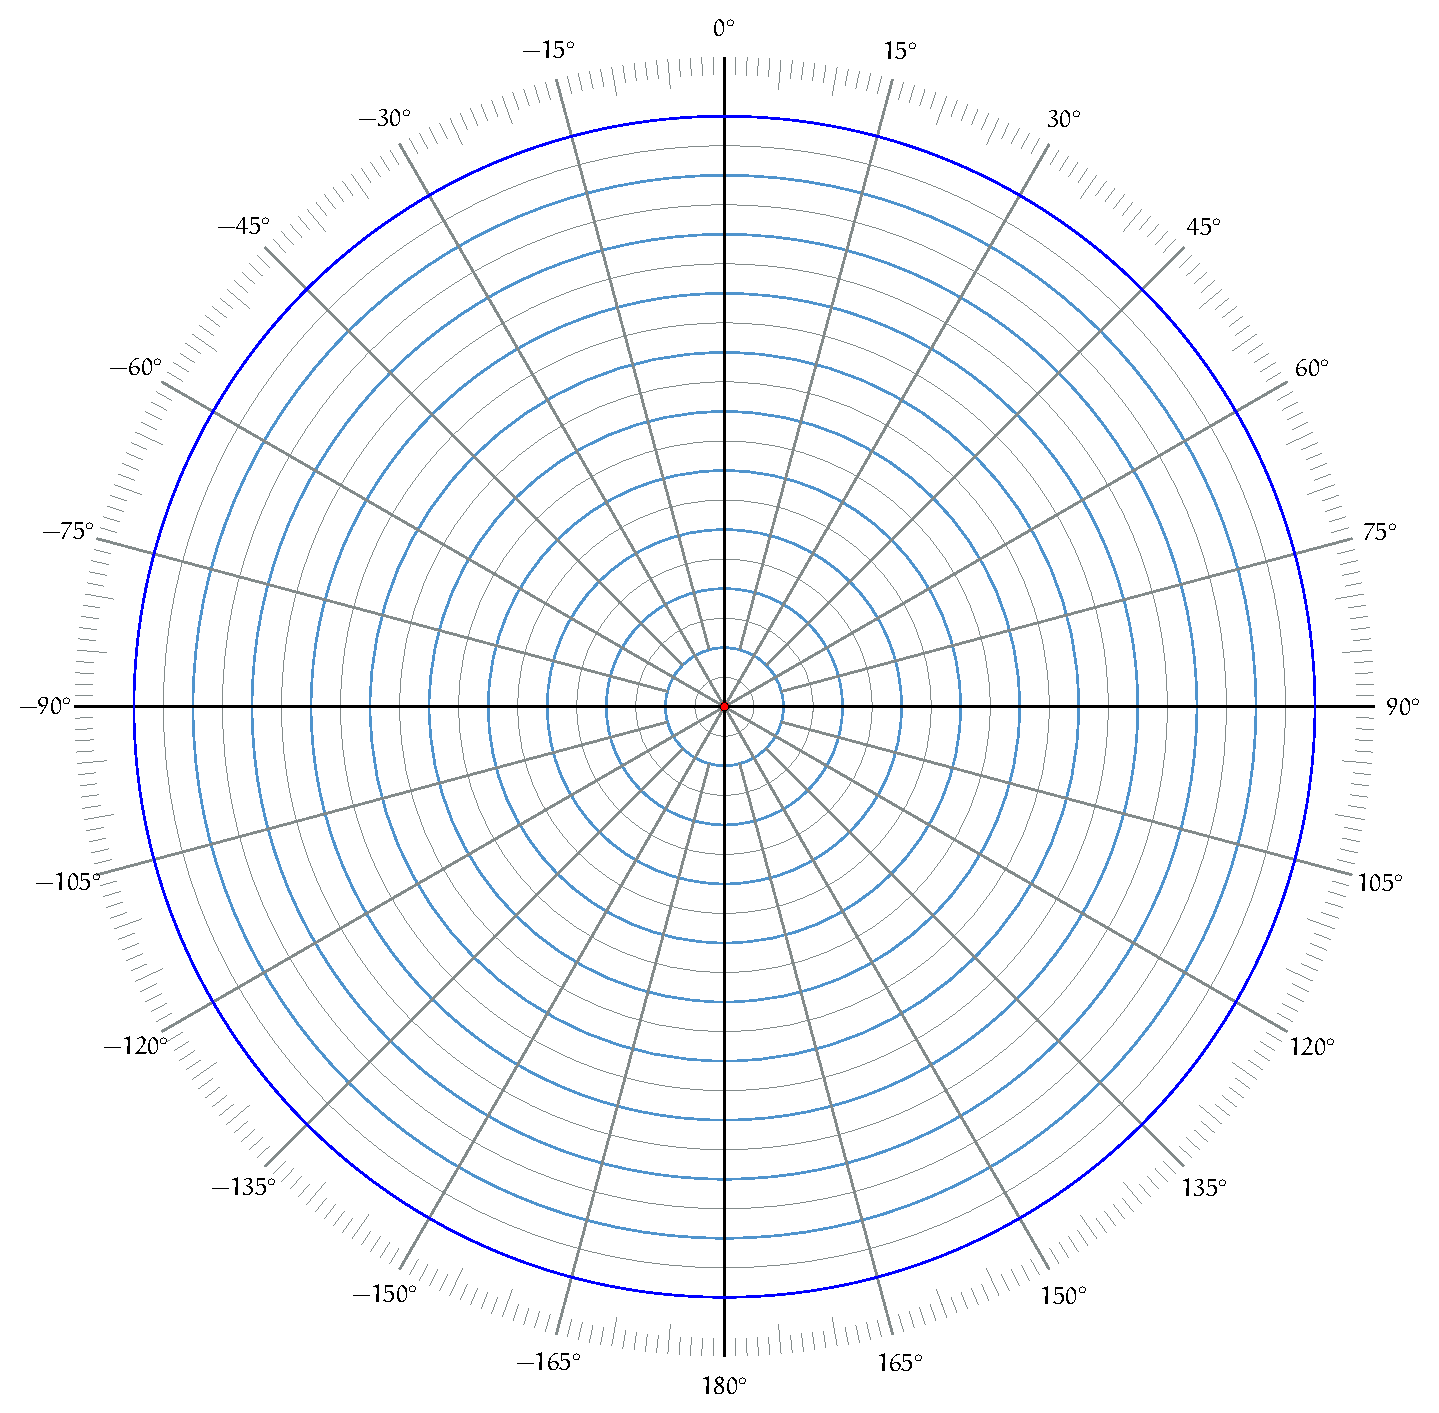
\includegraphics[width=1\columnwidth]{CAPITOLI/_TIKZ/POLAR/omni}
\caption{non-directional}
\label{fig:mspan}
\end{figure}

%Il disegno nella parte sinistra di fig. 8 rappresenta la struttura di un tipico microfono a pressione (pressure microphone) omnidirezionale, mentre nella parte destra è rappresentata la sua curva polare, dove vediamo che la direzionalità del suono inizia ad essere percepita dal microfono a partire da circa 5 KHz in su, mentre le frequenze gravi non sono indicate in quanto assimilabili a quella rilevata a 1 KHz, cioè con attenuazione zero per qualsiasi angolo di provenienza del suono.

Dalla descrizione di Blumlein di \emph{Mid-Side}, abbiamo un canale frontale
\emph{Mid} comunemente descritto da un microfono cardioide. Il microfono
cardioide del primo ordine potrebbe essere descritto come una somma delle
variazioni di pressione non direzionale (\emph{ndp})

and bidirectional pressure gradient variations.

\begin{equation}
bpg = x\cos\theta
\label{eq:fig8}
\end{equation}

\begin{figure}[h]
\centering
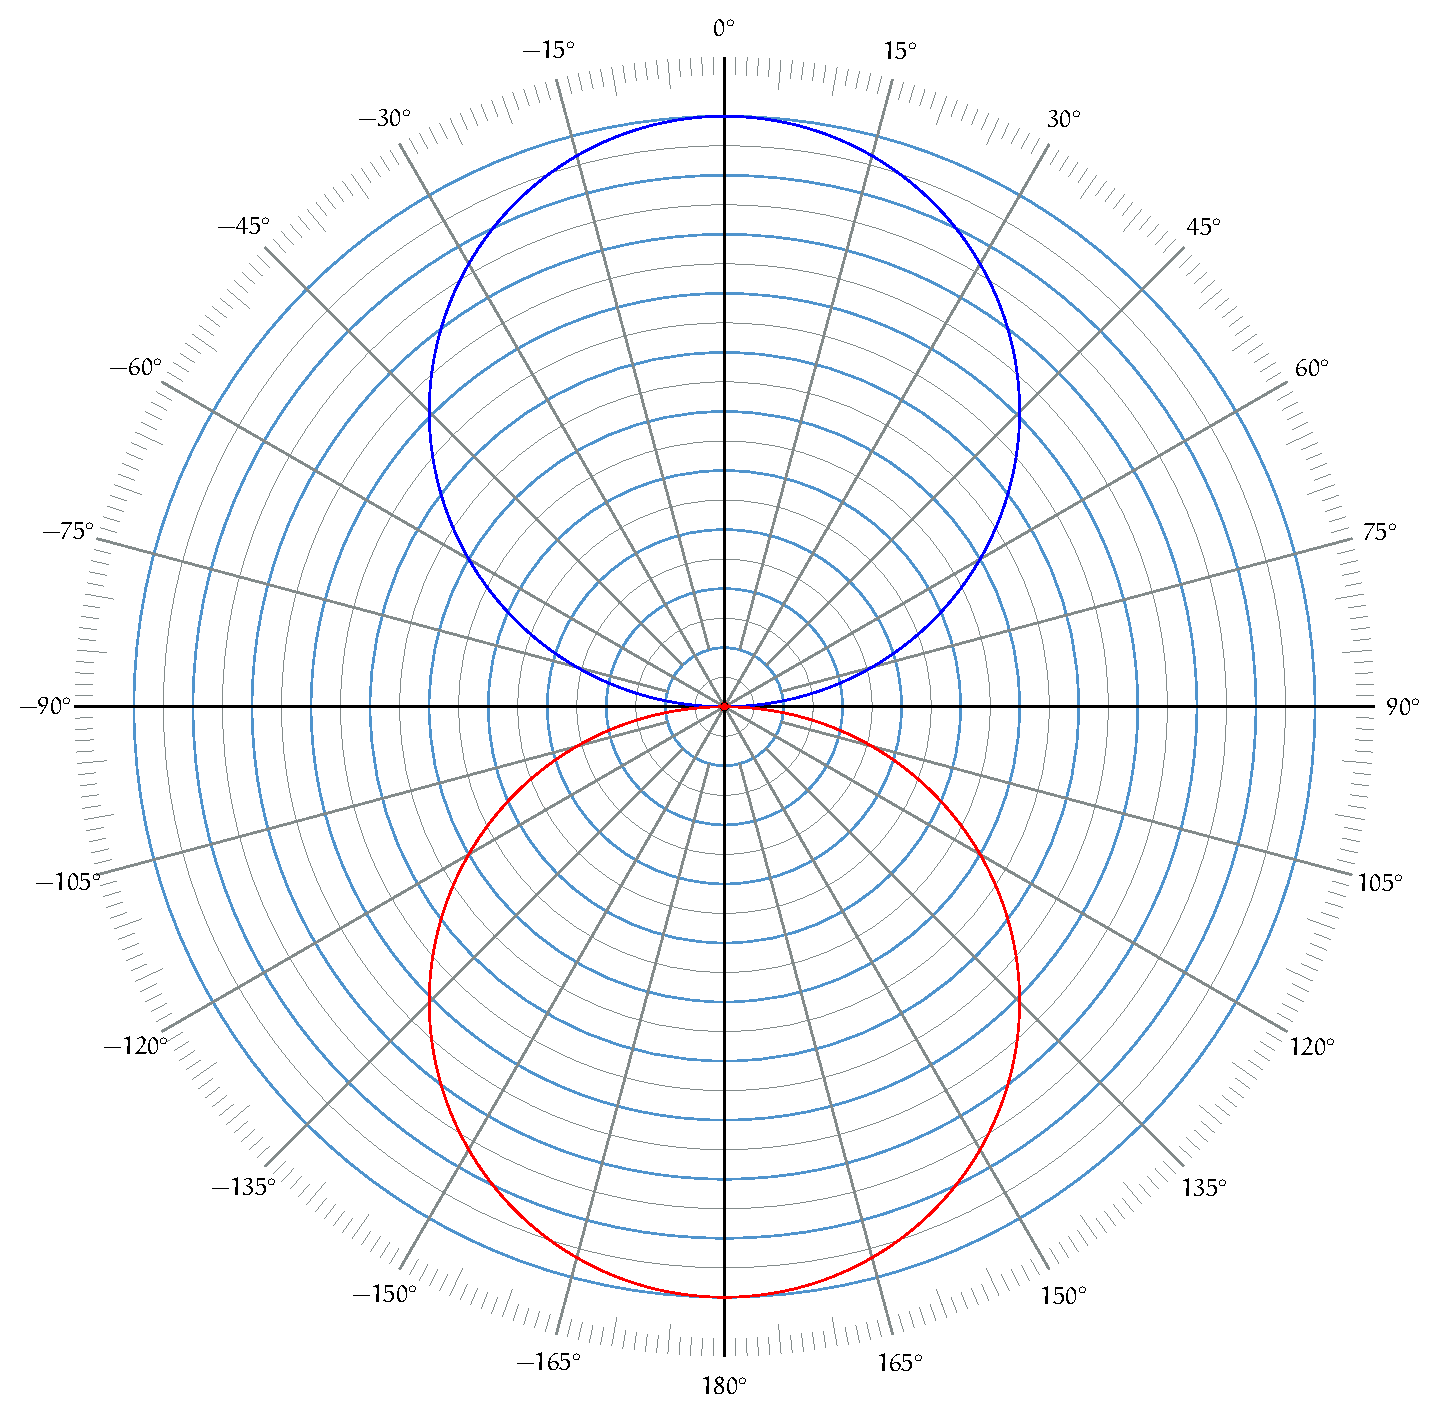
\includegraphics[width=1\columnwidth]{CAPITOLI/_TIKZ/POLAR/fig8}
\caption{Figure-8}
\label{fig:mspan}
\end{figure}

La prima differenza rilevante tra un'equazione del modello polare non
direzionale (\ ref {eq: omni}) e una direzionale (\ ref {eq: fig8}) è la
presenza del coefficiente angolare. L'angolo \ emph {theta} nell'equazione
(\ref{eq:fig8}) descrive la direzione di puntamento del microfono bidirezionale
espressa in radianti. $ X $ è il segnale relativo alla pressione.

Il microfono cardioide (\ emph {cpg}) che tentiamo di sintetizzare deve puntare
alla posizione centrale-anteriore che è il riferimento zero radianti.

\begin{equation}
cpg = 0.5(x) + 0.5(x\cos\theta)
\label{eq:cardioid}
\end{equation}

\begin{figure}[h]
\centering
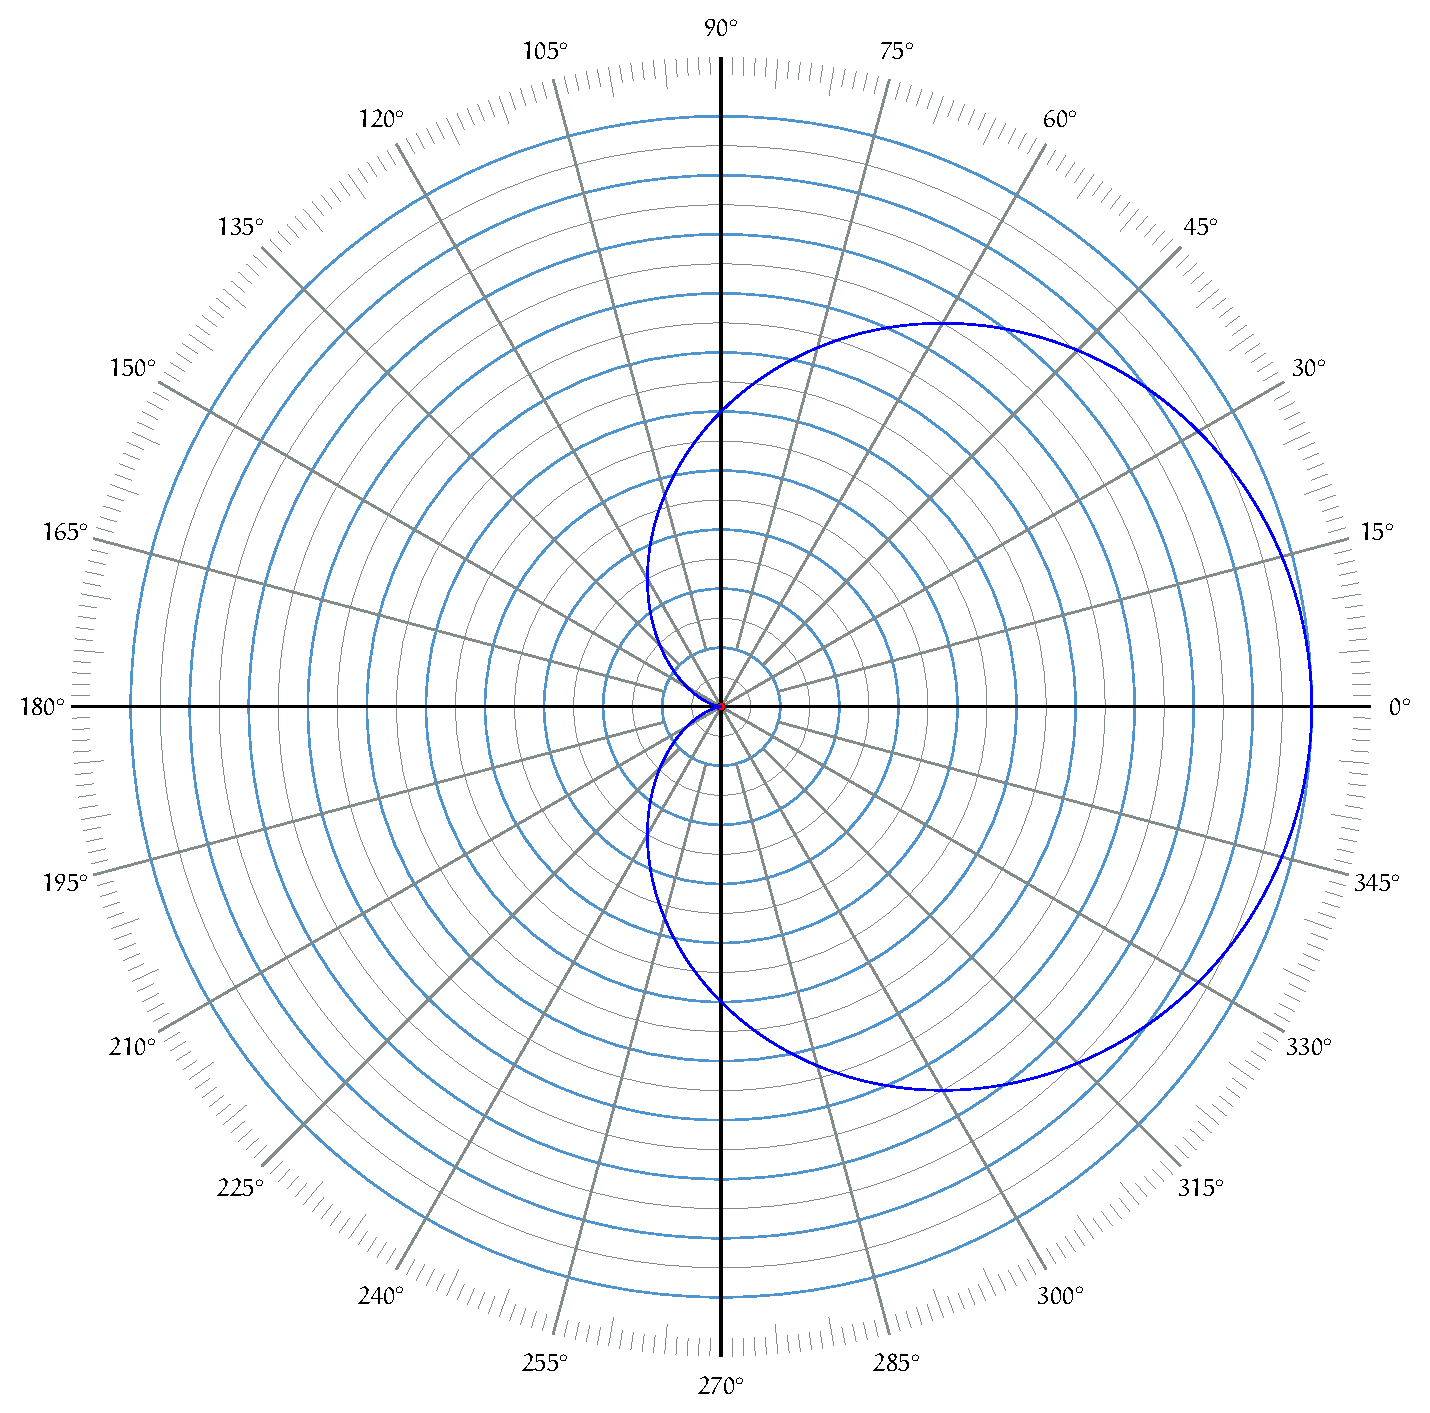
\includegraphics[width=1\columnwidth]{CAPITOLI/_TIKZ/POLAR/cardioid}
\caption{Cardioid}
\label{fig:mspan}
\end{figure}

Cardioidi e altri schemi più comuni del primo ordine sono prodotti con il
seguente peso tra la pressione non direzionale e il gradiente di pressione
bidirezionale:

\begin{table}[h]
\begin{center}
\begin{tabular}{cc}
Polar Pattern & Equation \\
\hline
Omnidirectional & $ 1(x) $ \\
Subcardioid     & $ 0.75(x) + 0.25(x\cos\theta) $ \\
Cardioid        & $ 0.5(x) + 0.5(x\cos\theta) $ \\
Supercardioid   & $ 0.37(x) + 0.63(x\cos\theta) $ \\
Hypercardioid   & $ 0.25(x) + 0.75(x\cos\theta) $ \\
Bidirectional   & $ 1(x\cos\theta) $ \\
\end{tabular}
\end{center}
\caption{coefficiente \emph{pressione non direzionale} e coefficiente
\emph{gradiente di pressione bidirezionale} per la descrizione dei modelli
polari del primo ordine. Dove $ x $ è il segnale di input, l'angolo di incidenza
della prospettiva $\theta$}
\label{tab:example}
\end{table}

Quindi dai primitivi schemi polari del primo ordine, non direzionali e
bidirezionali, potremmo derivare, progressivamente, ogni sfumatura di forma tra
di loro, puntando angolarmente ovunque intorno a 2 $ \ pi $ radianti.

Infine, il componente Mid del panner Mid-Side potrebbe essere espresso dalla
formula

\begin{equation}
m(x,p,\theta) = (p*x) + ((1-p)*(x\cos\theta)
\label{eq:mid}
\end{equation}

Dove $ x $ è il segnale di ingresso, $ p $ è il coefficiente di ampiezza, $0.5$
per scopi cardioidi, $\theta$ è la direzione di impatto angolare espressa in
radianti.

Il componente Side è la formula dritta bipolare di figura 8 che punta a sinistra.

\begin{equation}
s(x,\theta) = x*(sin(\theta))
\label{eq:mid}
\end{equation}

Il codice Faust per un panner Mid-Side è veramente auto-spiegato: le equazioni
diritte per descrivere sia il cardioide che la figura 8 sono i due componenti
al di fuori del panning.

%--------------------------------------------
%----------------larghezza massima del codice
\begin{lstlisting}
mspan(x,p,rad) = m,s
with{
  m = (p*x)+((1-p)*(x*cos(rad)));
  s = x*(sin(-rad));
};
\end{lstlisting}

\begin{figure}[h]
\centering
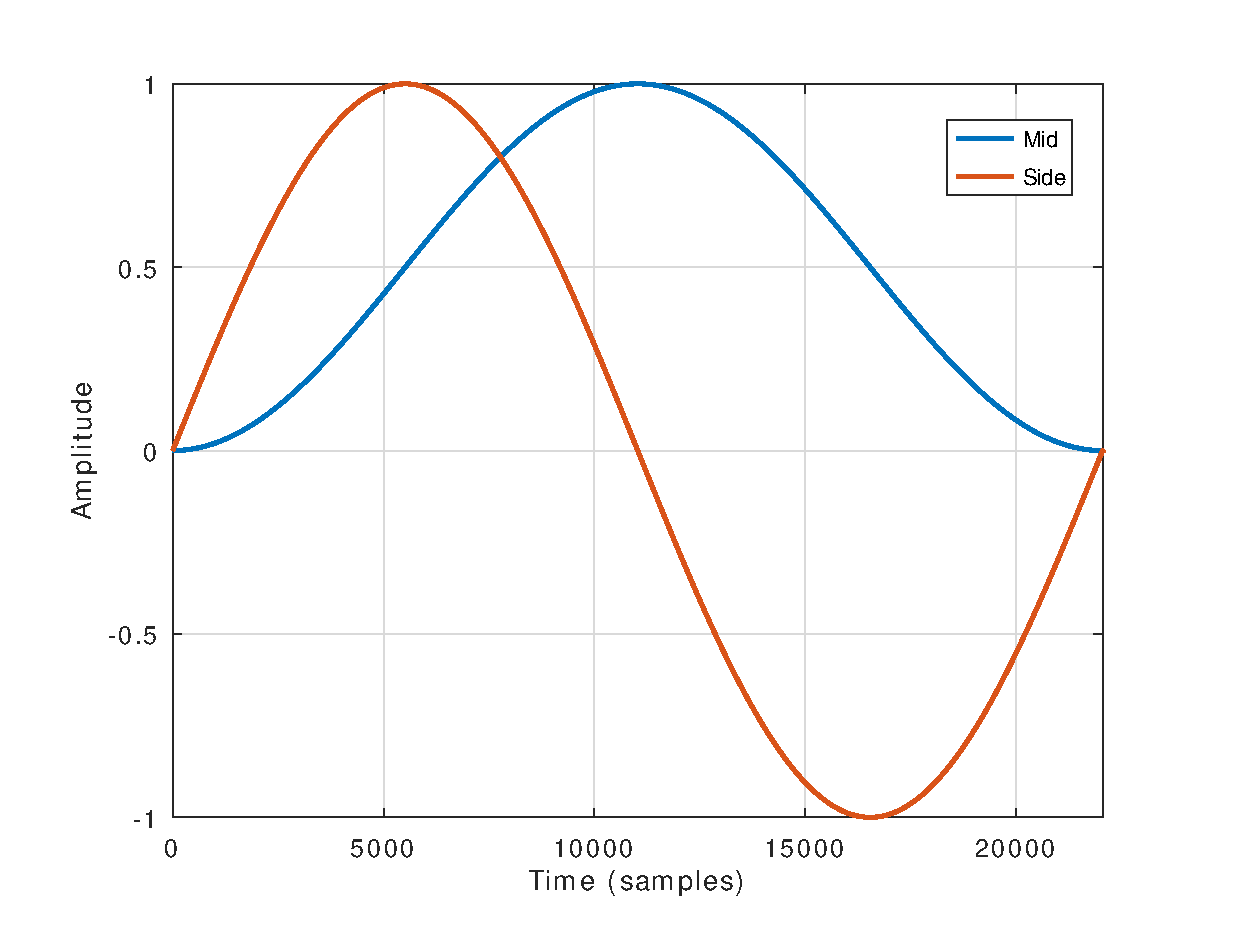
\includegraphics[width=1\columnwidth]{CAPITOLI/1000/IMG/mspan}
\caption{Mid-Side Panner. Il grafico mostra la risposta del panner ad una
variazione di 360 gradi da sinistra (-180 gradi) a destra (180 gradi). La linea
laterale (rossa) mostra la
bipolarità del segnale correlata alle informazioni angolari. La linea Mid (blu)
ha solo energia positiva in relazione alle informazioni angolari. La trama
mostra l'evidenza del significato zero su entrambi i bordi di -180 e 180 gradi,
dove cardioide e figura 8 sono senza ascolto.}
\label{fig:mspan}
\end{figure}

Dobbiamo passare il panner attraverso la matrice della differenza di somma per
ottenere ciò che Blumlein descrive come la differenza di ampiezza nei segnali
degli altoparlanti dalle differenze di fasi.

%--------------------------------------------
%----------------larghezza massima del codice
\begin{lstlisting}
mspan_lr(x,p,rad) = mspan(x,p,rad) : sdmx;
\end{lstlisting}

\section{MS-PAN Live usage}

Il panner Mid-Side qui proposto non è solo un oggetto tecnico, utile o no,
comparabile o no, relativo ad altri tipi di pan. Il panner Mid-Side qui proposto
è un oggetto di pensiero. Usiamo la tecnica Mid-Side, per riflettere la stessa
stereofonia; perché riteniamo fortemente che alcune circostanze evidenziate
nelle sezioni precedenti debbano essere affrontate, altre migliorate e molte
altre uccise.

Pensare al panning deve essere fortemente incoraggiato perché è un oggetto
semplice troppo spesso usato senza fare domande. La gente può pensare che la
chiave quadratica sia migliore di quella lineare che solo in virtù della sua
introduzione più recente. Ma se interrompiamo il suo “utilizzo senza mettere in
discussione” e, come musicisti, prendiamo il tempo per analizzare l'uso manuale
dell'uno al posto dell'altro, possiamo sentire una differenza, pratica prima del
suono.

Conoscendoli possiamo analizzare il mercato del mixer e il ruolo del pan nella
musica di cultura di massa. Senza un \ -a \ -lys \ -ing questi problemi pratici,
non è davvero comprensibile il motivo per cui la peggiore tecnica di panning sia
mai la maggior parte dell'hardware implementato.

Il codice per costruire un panner di ampiezza quadratica è piuttosto banale.
Il codice più prolisso \ emph {Faust} lo farà in cinque righe. L'eliminazione di
$sqrt$ dalle seguenti formule diventa il panner di ampiezza lineare tradizionale
più semplice.

%--------------------------------------------
%----------------larghezza massima del codice
\begin{lstlisting}
lrpanq(x,p) = l,r
with{
  l = sqrt(1-p)*x;
  r = sqrt(p)*x;
};
\end{lstlisting}

Dove $ p $ è il coefficiente angolare espresso dal potenziometro, in un
intervallo tra $ 0 $ la posizione sinistra, $ 0,5 $ la posizione centrale e $1$
la posizione destra.

Sorridendo, potrebbe essere fatto su una riga:

%--------------------------------------------
%----------------larghezza massima del codice
\begin{lstlisting}
lrpanq(p) = _ <: sqrt(1-p)*_, sqrt(p)*_;
\end{lstlisting}

\begin{figure}[t]
\centering
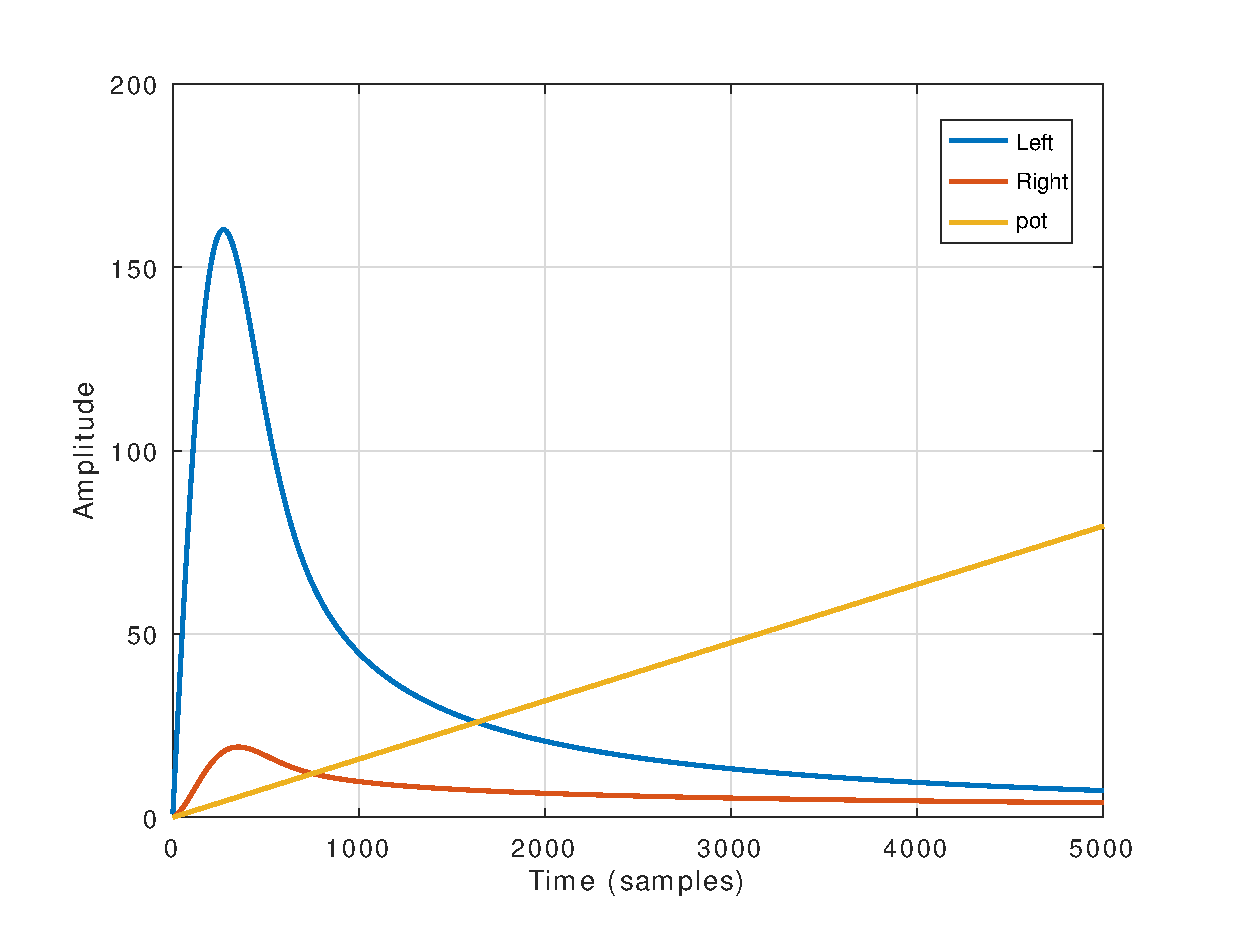
\includegraphics[width=1\columnwidth]{CAPITOLI/1000/IMG/lrpanfb_init}
\caption{\textbf{Risposta feedback panner ampiezza quadratica sinistra-destra}.
La trama mostra la risposta del programmatore in un ciclo di scansione da
sinistra a destra. La trama mostra come l'ampiezza si sposta rapidamente oltre
150 volte il valore iniziale sul canale “in feedback” e oltre 20 volte sul
canale “opposto”.}
\label{fig:lrpanfb1}
\end{figure}

\begin{figure}[t]
\centering
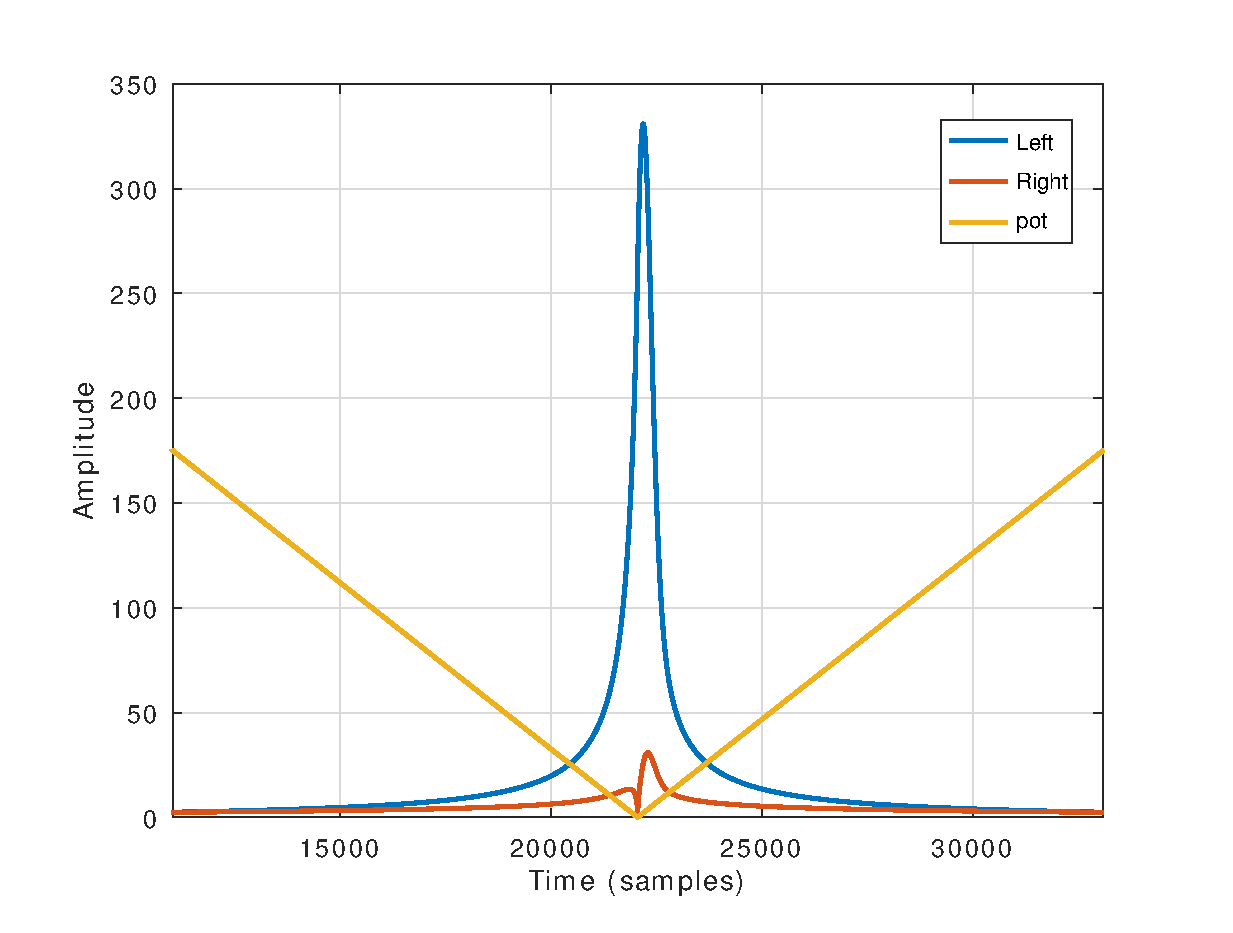
\includegraphics[width=1\columnwidth]{CAPITOLI/1000/IMG/lrpanfbpot2}
\caption{\textbf{Risposta feedback panner ampiezza quadratica sinistra-destra}.
La trama mostra la risposta del programmatore in un ciclo di scansione da
sinistra a destra. La trama mostra come l'ampiezza si sposta rapidamente oltre
150 volte il valore iniziale sul canale “in feedback” e oltre 20 volte sul
canale “opposto”.}
\label{fig:lrpanfb2}
\end{figure}

Abbiamo spiegato il percorso del pan Mid-Side, partendo dalle radici. Ora è il
momento di capire quali sono i possibili utilizzi e quali sono le peculiarità di
un panner Mid-Side invece dei pannolini di ampiezza \emph{tradizionale}.

Il segnale \emph{matrixed} ha la sua complessità come svantaggio. Fermare. In
realtà richiede conoscenza e fantasia per comprendere un segnale come il
significato della combinazione di matrici e richiede anche un po 'di lavoro
complicato più di un segnale diretto.

Come musicisti, anche quando trame e formule appaiono abbastanza chiare, alla
fine, al momento del giudizio, sono le orecchie e l'usabilità musicale a
determinare la scelta migliore, personale.

L'affascinante regno dei segnali \ emph {matrixed} costringe un po 'a lavorare
con il pensiero. Quindi, per noi, ad esempio, la forza di modulazione di fase
del panner Mid-Side aveva suggerito, anche prima di un test pratico, una
migliore stabilità sugli utilizzi dal vivo. Perché? È abbastanza semplice da
dimostrare.

Un microfono viene instradato in un canale, con una chiave appuntita a metà
laterale, supponiamo che 23 gradi a sinistra e inviato agli altoparlanti. Con il
panner quadratico, entrambi i canali sinistro e destro hanno valori di ampiezza
diversi con gli stessi valori di fase. Il feedback dei segnali degli
altoparlanti all'interno del microfono proviene da diverse fonti di energia in
fase. La ricerca del feedback con le dita sul guadagno produrrà segnali che
aumenteranno almeno quadraticamente [fig. \ref{fig:lrpanfb1}, \ref{fig:lrpanfb2}].

\begin{figure}[h]
\centering
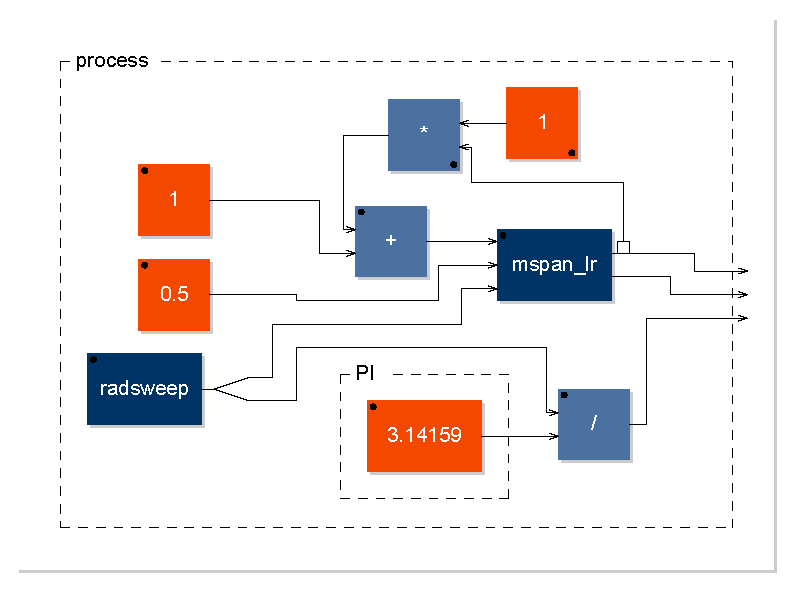
\includegraphics[width=1\columnwidth]{CAPITOLI/1000/IMG/mspanlrfb_diagram}
\caption{\textbf{Block diagram of the infinite feedback}.}
\label{fig:mspan}
\end{figure}

D'altra parte, nella stessa situazione di feedback, con la stessa provenienza
del panning angolare applicata al segnale del microfono, il pan Mid-Side
produrrà fasi diverse e energia diversa per entrambi gli altoparlanti. Le
differenze, nell'aria, produrranno un modello di feedback più resistivo. In
altre parole, il panner di Mid-Side agisce “naturalmente” come anti-\emph{Larsen}.


\begin{figure}[t]
\centering
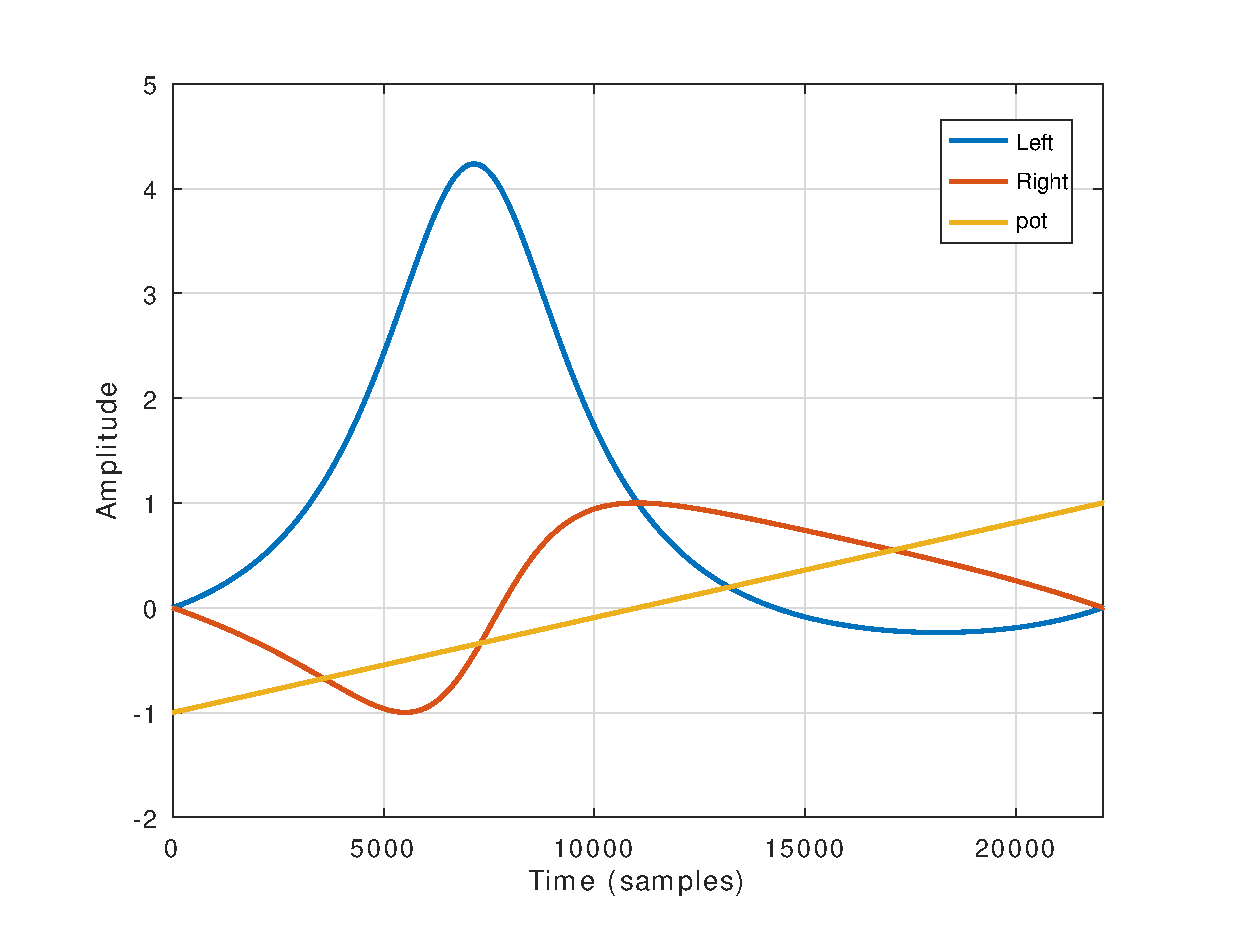
\includegraphics[width=1\columnwidth]{CAPITOLI/1000/IMG/mspanlrfbpot}
\caption{\textbf{Mid-Side to Left-Right panner}. The plot describes the feedback
response with a pan movement through the entire panorama, from -180 to 180
degrees (yellow line, normalized to -1 and 1). The energy multiplies up to four
times for the left channel in infinite feedback (blue line). The top of feedback
increasing is at 45 degrees position in direction of the channel in feedback.}
\label{fig:mspanlrfb}
\end{figure}
